\documentclass[twocolumn]{article}
\usepackage{amsmath, amssymb, graphicx, hyperref, cuted}

\title{Pond Ecosystem}
\author{Purva Parmar \\ 20181081}
\date{}

\renewcommand{\familydefault}{\sfdefault}

\begin{document}

\graphicspath{{../}}
\setlength{\parindent}{0pt}
\setlength{\parskip}{\baselineskip}

\maketitle

%\begin{strip}
 %   \tableofcontents
 %   \vspace{3em}
%\end{strip}

\section{Aim}
To study a pond sample ecosystem in a Winogradsky Column and analyze the Diversity 

\section{Theory}

\subsection{Biodiversity}

Biodiversity is the variability present in living organisms in an ecosystem.

We can quantify diversity through certain means. 

\begin{itemize}
    \item \textbf{Alpha Diversity}: $\alpha$-diversity simply refers to the number of species for a given ecosystem.
    \item \textbf{Beta Diversity}: $\beta$-diversity is a comparison between two ecosystems or areas, considering their area size and local effects
\end{itemize}

We will look at some $\alpha$-diversity indices.

\subsubsection{Alpha Diversity}

\begin{itemize}
    \item \textbf{Number of species}
    
    The number of species $S$ gives a simple measure of the diversity. More the number of species, the greater is the diversity.

    \item \textbf{Richness (Margalef)}
    
    The Margalef Index ($R_{Mg}$) is defined by:

    \[
        \sf R_{Mg} = \frac{S-1}{\ln N} 
    \]

    where $N$ is the total number of individuals in the population.

    A higher Margalef Index value suggests a higher diversity.

    \item \textbf{Simpson's Index}
    
    The Simpson's Index is:

    \[
        \sf \lambda = \sum_{i=1}^{S} P_i^2
    \]

    where $P_i = \dfrac{n_i}{N}$.

    The Simpson's Diversity Index becomes:

    \[ 
        \sf D = 1 - \lambda    
    \]

    Here, $P_i^2$ refers to the Probability of finding the same organism again and again. So, the summation gives an inverse idea of diversity.

    We subtract it from 1 for an index of diversity.

    The Simpson's Index does not account for rare species well.

    \item \textbf{Shannon's Index}
    
    \[ 
        \sf H' = -\sum_{i=1}^{S}P_i \ln P_i    
    \]

    $H'$ attains maximum value when all species are equally dominant. In this case, $P_i = \dfrac{1}{S}$ and hence:

    \[ 
        \sf H_{max}' = \ln S    
    \]

    The Shannon's Index only compares species numbers. For smaller areas, the Shannon's Index will be smaller. 

    \item \textbf{Evenness}
    
    Evenness normalizes Shannon's Index.

    \[
        \sf E = \frac{H'}{\ln S}    
    \]

    Hence, $0 \leqslant E \leqslant 1$. This helps us compare systems of different sizes.

    \item \textbf{Berger-Parker Index}
    
    The Berger-Parker Index simply takes the fraction of the most dominant species in the sample.

    \[ 
        \sf BP = \frac{n_{max}}{N}    
    \]

    where $\sf n_{max}$ refers to the population size of the most dominant species. 

    If the BP Index is large, it shows that the area is heavily dominated by a single species and that diversity might be low. There are more species which are rare.

    \item \textbf{Hill Number}
    
    There is a formula, with a parameter $a$. Different values of $a$ gives the different indices above.
    
    \begin{center}
    \begin{tabular}{c|c}
        \textbf{a} & \textbf{Index} \\ \hline
        0 & S \\
        1 & $\sf \lambda$ \\
        2 & H' \\
        $\infty$ & BP
    \end{tabular}
    \end{center}
\end{itemize}

\subsection{Experimetal Observations}

\subsubsection{OTUs and their Frequencies}

\begin{center}
\begin{tabular}{|c|c|c|c|}
\hline
\textbf{OTU} & \textbf{Week 0} & \textbf{Week 3} & \textbf{Week 11} \\ \hline
1             & 1               & 30              & 7                \\ \hline
2             & 200             & 1               & 1                \\ \hline
3             & 1               & 1               & 100              \\ \hline
4             & 3               & 6               & 4                \\ \hline
5             & 42              & 6               & 100              \\ \hline
6             & 6               & 1               & 4                \\ \hline
7             & 44              & 1               & 12               \\ \hline
8             & 11              & 1               & 1                \\ \hline
9             & 1               & 1000            & 20               \\ \hline
10            & 2               &                 & 2                \\ \hline
11            & 1               &                 &                  \\ \hline
12            & 9               &                 &                  \\ \hline
13            & 2               &                 &                  \\ \hline
14            & 39              &                 &                  \\ \hline
15            & 2               &                 &                  \\ \hline
16            & 1               &                 &                  \\ \hline
17            & 1               &                 &                  \\ \hline
18            & 11              &                 &                  \\ \hline
19            & 2               &                 &                  \\ \hline
20            & 1               &                 &                  \\ \hline
21            & 4               &                 &                  \\ \hline
\end{tabular}
\end{center}

\subsubsection{Chemical Analysis}

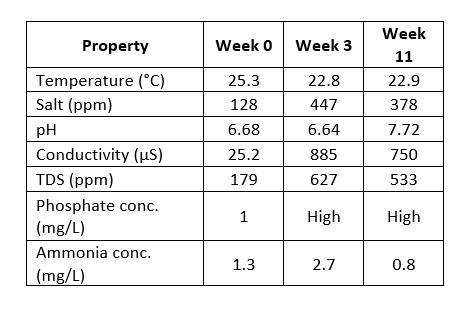
\includegraphics[width = \linewidth]{Pond Ecosystem Chemical Analysis.png}

\subsubsection{Diversity Indices}

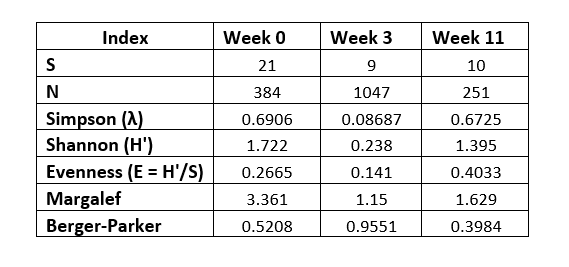
\includegraphics[width = \linewidth]{Diversity Indices.png}

\section{Inferences and Analysis}

The water was initially dirty and mostly filled with lower orgnisms.

We had diatoms, cyanobacteria, a lot of spirochaetes. 

In Week 3, a lot of ciliates were seen. These feed on sulphide producing bacteria, which grow in anoxic conditions. The water was blackish and smelled of $H_2S$.


The Week 11 column was clear water. On observations, we found mostly higher level organisms. Cyclops was seen. 

The primary producers were not to be seen. The low productivity of primary producers, which may have lead to the reduction in number of lower organisms.

The number of lower organisms had been high previously, which explains presence of higher level organisms.


\textbf{Diversity}

The Burger-Parker Index in Weeks 0 and 3 are quite high, which is in accordance with the high numbers of the dominant species. 

Week 11 showed better diversity compared to the previous weeks, even though the total number of organisms, N, was low.

This is also reflected in the Evenness, which is (in my way of thinking) normalized Shannon's Index. 

Overall, the number of species observed remained similar in Weeks 3 and 11. 

\end{document}